%=== Câu 1 (ID: None) ===%

\nguon{nhóm Latex}
\dang{Ôn tập đề  1}
\begin{ex}
	Cho $x$ là một phần tử của tập hợp $X$. Mệnh đề nào sau đây là $\textbf{đúng}$?
	\choice
	{\True $x \in X$}
	{$X \in x$}
	{$x \subset X$}
	{$\{x\} \in X$}
	\loigiai{
		Mệnh đề là đúng là $x \in X$. Kí hiệu $x$ là một phần tử của tập hợp $X$.
	}
\end{ex}

%=== Câu 2 (ID: None) ===%

\nguon{nhóm Latex}
\dang{Ôn tập đề  1}
\begin{ex}
	Cho tập hợp $A=\{x \mid x \in \mathbb{N}, x \leq 5\}$. Số phần tử của tập hợp $A$ là
	\choice
	{$8$}
	{$7$}
	{$5$}
	{\True $6$}
	\loigiai{
		$A=\{x \mid x \in \mathbb{N}, x \leq 5\} \Leftrightarrow A=\{0; 1 ; 2 ; 3 ; 4 ; 5\}$. Do đó số phần tử của tập hợp $A$ là $6$.
	}
\end{ex}

%=== Câu 3 (ID: None) ===%

\nguon{nhóm Latex}
\dang{Ôn tập đề  1}
\begin{ex}
	Cho tập hợp $X=\{0 ; 2 ; 5\}$. Tập hợp nào dưới đây $\textbf{không}$ phải là tập con của tập hợp $X$?
	\choice
	{$\varnothing$}
	{$\{2\}$}
	{$\{0 ; 2 ; 5\}$}
	{\True  $\{0 ; 1 ; 2\}$}
	\loigiai{
		Ta có $1 \notin X$,  vậy $\{0 ; 1 ; 2\} \not \subset\{0 ; 2 ; 5\}$.
	}
\end{ex}

%=== Câu 4 (ID: None) ===%

\nguon{nhóm Latex}
\dang{Ôn tập đề  1}
\begin{ex}
	Số phần tử của tập $C=\{x \in \mathbb{Z} \mid-1 \leqslant x \leqslant 1\}$ là
	\choice
	{\True $3$}
	{$2$}
	{$1$}
	{$6$}
	\loigiai{
		Ta có $C=\{-1 ; 0 ; 1\}$ nên $C$ có $3$ phần tử.
	}
\end{ex}

%=== Câu 5 (ID: None) ===%

\nguon{nhóm Latex}
\dang{Ôn tập đề  1}
\begin{bt}
	Cho ba tập hợp $A=\{2; 5\}$, $B=\{5 ; x\}$, $C=\{x ; y ; 5\}$, biết $A=B=C$. Biết $x \neq y$, khi đó giá trị $x + y$ bằng
	\shortans{7}
	\loigiai{
		Vì $A=B$ nên $x=2$. Lại có $B=C$ nên $y=5$.\\
		Vậy $x+y=2+5=7$.
	}
\end{bt}

%=== Câu 6 (ID: None) ===%

\nguon{nhóm Latex}
\dang{Ôn tập đề  1}
\begin{ex}
	Cho tập $M=\{x \in \mathbb{R} \mid (x+3)(x-1) \geqslant 0\}$. Khi đó
	\choice
	{$M=(-\infty ;-1] \cup[3 ;+\infty)$}
	{\True  $M=(-\infty ;-3] \cup[1 ;+\infty)$}
	{$M=[1 ;+\infty)$}
	{$M=(-\infty ;-3]$} 
	\loigiai{
		Ta có $(x+3)(x-1) \geqslant 0 \Leftrightarrow \hoac{& x \leqslant-3  \\&  x \geqslant 1} $
		$\Rightarrow M=(-\infty ;-3] \cup [1 ;+\infty)$.
	}
\end{ex}

%=== Câu 7 (ID: None) ===%

\nguon{nhóm Latex}
\dang{Ôn tập đề  1}
\begin{bt}
	Cho hai tập hợp $A=\{n \in \mathbb{N} \mid-2<n \leqslant 4\}$ và $B=\{-1 ; 0\}$. Hãy xác định tập hợp $A \cap B$, $A \setminus B$.
	\loigiai{
		Ta có $A=\{0 ; 1 ; 2 ; 3 ; 4\}$, $B=\{-1 ; 0\}$.\\
		Suy ra $A \cap B=\{0\}$ và $A \setminus B=\{1 ; 2 ; 3 ; 4\}$.
	}
\end{bt}

%=== Câu 8 (ID: None) ===%

\nguon{nhóm Latex}
\dang{Ôn tập đề  1}
\begin{ex}
	Trong các tập hợp sau, tập hợp nào là tập hợp rỗng?
	\choice
	{$A=\{x \in \mathbb{Z}|~ x<1\}$}
	{$B=\left\{x \in \mathbb{Z} \mid 6 x^2-7 x+1=0\right\}$}
	{\True $C=\left\{x \in \mathbb{Q} \mid x^2-4 x+2=0\right\}$}
	{$D=\left\{x \in \mathbb{R} \mid x^2-4 x+3=0\right\}$}
	\loigiai{
		\begin{itemize}
			\item Ta có $x^2-4 x+2=0 \Leftrightarrow \hoac{& x=2+\sqrt{2} \notin \mathbb{Q}  \\&  x=2-\sqrt{2} \notin \mathbb{Q}} \Rightarrow C=\varnothing$.
			\item $A=\{x \in \mathbb{Z}|~ x<1\} = \{ \cdots;-3;-2;-1;0 \} \neq \varnothing$.
			\item $6x^2-7x+1=0 \Leftrightarrow \hoac{&x=1 \in \mathbb{Z}\\&x=\dfrac{1}{6} \notin \mathbb{Z}} \Rightarrow B = \{ 1 \}$.
			\item $x^2-4x+3=0 \Leftrightarrow \hoac{&x=3 \in \mathbb{R} \\&x=1 \in \mathbb{R}} \Rightarrow D = \{ 1;3 \}$.
		\end{itemize}
	}
\end{ex}

%=== Câu 9 (ID: None) ===%

\nguon{nhóm Latex}
\dang{Ôn tập đề  1}
\begin{ex}
	Cho tập hợp $B=\left\{ x\in\mathbb{Z}\mid x^4-11x^2+18=0\right\}$. Khi đó số phần tử của tập hợp $B$ là
	\choice
	{$1$}
	{\True $2$}
	{$3$}
	{$4$}
	\loigiai{
		Ta có 
		\[
		x^4-11 x^2+18=0
		\Leftrightarrow \hoac{&x^2=2\\& x^2=9}
		\Leftrightarrow \hoac{&x=\sqrt{2}\notin\mathbb{Z}\\& x=-\sqrt{2}\notin\mathbb{Z}\\& x=3\in\mathbb{Z}\\& x=-3 \in \mathbb{Z}.}
		\]
		Vậy $B=\{-3 ; 3\}$ nên $B$ gồm $2$ phần tử.
	}
\end{ex}

%=== Câu 10 (ID: None) ===%

\nguon{nhóm Latex}
\dang{Ôn tập đề  1}
\begin{ex}
	Cho các tập hợp $A=\{-3 ;-2 ;-1 ; 0 ; 1 ; 2 ; 3\}$, $B=\{0 ; 1 ; 4 ; 5\}$ và $C=\{-4 ;-3 ; 1 ; 2 ; 5 ; 6\}$.
	\choiceTF[1]
	{\True $A\cup B=\{-3 ;-2 ;-1 ; 0 ; 1 ; 2 ; 3 ; 4 ; 5\}$}
	{$A\cap B=\{0\}$}
	{\True $(A\cup B)\cap C=\{-3 ; 1 ; 2 ; 5\}$}
	{\True $A\cap B\cap C=\{1\}$}
	\loigiai{
		\begin{itemchoice}
			\item Vì $A\cup B=\{-3 ;-2 ;-1 ; 0 ; 1 ; 2 ; 3 ; 4 ; 5\}$.
			\item Vì $A\cap B=\{0 ; 1\}$.
			\item Vì $(A\cup B)\cap C=\{-3 ; 1 ; 2 ; 5\}$.
			\item Vì $A\cap B\cap C=\{1\}$.
		\end{itemchoice}
	}
\end{ex}

%=== Câu 11 (ID: None) ===%

\nguon{nhóm Latex}
\dang{Ôn tập đề  1}
\begin{ex}
	Cho $A=[-1 ; 3]$; $B=(2 ; 5)$. Tìm mệnh đề \textbf{sai}.
	\choice
	{$B \setminus A=(3 ; 5)$}
	{$A \cap B=(2 ; 3]$}
	{$A \setminus B=[-1 ; 2]$}
	{\True  $A \cup B=[-1 ; 5]$}
	\loigiai{
		\begin{center}
			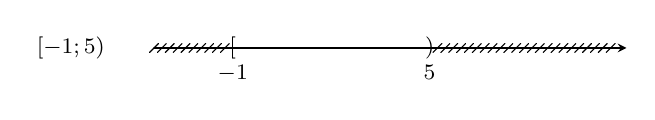
\begin{tikzpicture}[scale=1,>=stealth, font=\footnotesize, line join=round, line cap=round]
				\draw [-stealth] (0,0)--(6,0);
				\path (1,0) node{$[$} (1,-0.1)node[below]{$-1$} (-.5,0)node[left]{$[-1 ;5)$};
				\path (3.5,0) node{$)$} (3.5,-0.1)node[below]{$5$};
				\foreach \x in{0,0.1,...,1} \draw (\x,0)--++(45:.08) (\x,0)--++(-135:.08);
				\foreach \x in{3.6,3.7,...,5.8} \draw (\x,0)--++(45:.08) (\x,0)--++(-135:.08);
			\end{tikzpicture}
		\end{center}
		Ta có $A \cup B=[-1 ; 5)$.
	}
\end{ex}

%=== Câu 12 (ID: None) ===%

\nguon{nhóm Latex}
\dang{Ôn tập đề  1}
\begin{ex}
	Cho tập $A=\{0 ; 2 ; 4 ; 6 ; 8\}$; $B=\{3 ; 4 ; 5 ; 6 ; 7\}$. Tập $A \setminus B$ là
	\choice
	{$\{0 ; 6 ; 8\}$}
	{\True $\{0 ; 2 ; 8\}$}
	{$\{3 ; 6 ; 7\}$}
	{$\{0 ; 2\}$}
	\loigiai{
		Vì $A \setminus B$ gồm các phần tử thuộc tập hợp $A$ và không thuộc $B$ nên $A \setminus B=\{0 ; 2 ; 8\}$.
	}
\end{ex}

%=== Câu 13 (ID: None) ===%

\nguon{nhóm Latex}
\dang{Ôn tập đề  1}
\begin{ex}
	Cách viết nào sau đây là \textbf{sai}?
	\choice
	{$(0 ;+\infty)=\{x \in \mathbb{R}| x>0\}$}
	{$[0 ; 5]=\{x \in \mathbb{R}| 0 \leqslant x \leqslant 5\}$}
	{$(0 ; 5)=\{x \in \mathbb{R}| 0<x<5\}$}
	{\True $[-1 ; 5)=\{-1 ; 0 ; 1 ; 2 ; 3 ; 4\}$}
	\loigiai{
		Vì $[-1 ; 5)=\{x \in \mathbb{R} \mid -1 \leqslant x<5\}$ nên cách viết sau là sai: \lq\lq$[-1 ; 5)=\{-1 ; 0 ; 1 ; 2 ; 3 ; 4\}$\rq\rq.
	}
\end{ex}

%=== Câu 14 (ID: None) ===%

\begin{ex}
	\immini{
		Cho các tập hợp $A$, $B$, $X$ được biểu diễn trong biểu đồ Venn như sau. Khẳng định nào sau đây \textbf{sai}?
		\choice
		{$B \subset C_X A$}
		{$A \cap B=\varnothing$}
		{$A \subset C_X B$}
		{\True $A \cup B=X$}
	}{
		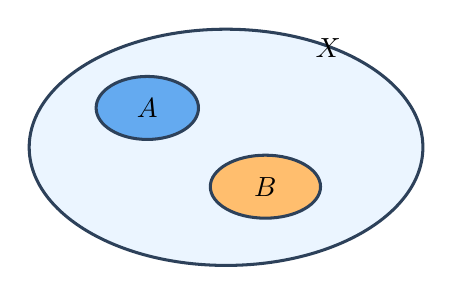
\begin{tikzpicture}[
			scale=0.5,
			thick,
			rotate=-90
		]
			% ===== MÀU SẮC =====
			\definecolor{MauNenX}{RGB}{235,245,255}
			\definecolor{MauA}{RGB}{100,170,240}
			\definecolor{MauB}{RGB}{255,190,110}
			\definecolor{MauVien}{RGB}{45,65,90}

			% ===== CÁC TẬP HỢP =====
			\def\ElipA{(0,0) ellipse (0.8cm and 1.3cm)}
			\def\ElipB{(2,3) ellipse (0.8cm and 1.4cm)}
			\def\ElipC{(1,2) ellipse (3cm and 5cm)}

			% ===== MIỀN X =====
			\fill[MauNenX] \ElipC;

			% ===== MIỀN A VÀ B =====
			\fill[MauA] \ElipA;
			\fill[MauB] \ElipB;

			% ===== ĐƯỜNG VIỀN =====
			\draw[MauVien,line width=1.1pt]
				\ElipC
				node[black,above right=1cm] {$X$};

			\draw[MauVien,line width=1.1pt]
				\ElipA
				node[black] {$A$};

			\draw[MauVien,line width=1.1pt]
				\ElipB
				node[black] {$B$};

		\end{tikzpicture}
	}
	\loigiai{
		Nhìn biểu đồ, ta thấy
		\[
			A\cup B\neq X.
		\]
		Vậy khẳng định sai là $A\cup B=X$.
	}
\end{ex}

%=== Câu 15 (ID: None) ===%

\nguon{nhóm Latex}
\dang{Ôn tập đề  1}
\begin{ex}
	Cho tập hợp $A=\{x \in \mathbb{R} \mid 2 \leqslant x<5\}$. Phần bù của tập hợp $A$ trong $\mathbb{R}$ là tập nào sau đây?
	\choice
	{$[5 ;+\infty)$}
	{$(-\infty ; 2)$}
	{$(-\infty ; 2] \cup(5 ;+\infty)$}
	{\True $(-\infty ; 2) \cup[5 ;+\infty)$}
	\loigiai{
		Ta có $A = \{x \in \mathbb{R} \mid 2 \leqslant x<5\} 
		= [2;5)$.\\
		Khi đó phần bù của tập hợp $A$ trong $\mathbb{R}$ là 
		$\mathrm{C_{\mathbb{R}}A}
		= \mathbb{R} \setminus A = (-\infty ; 2) \cup[5 ;+\infty)$.
	}
\end{ex}

%=== Câu 16 (ID: None) ===%

\nguon{nhóm Latex}
\dang{Ôn tập đề  1}
\begin{bt}Lớp 10A có $45$ học sinh trong đó có $12$ bạn học sinh giỏi Văn, $ 9$ bạn học sinh giỏi Địa lí, và $30$ bạn không giỏi môn học nào trong hai môn Văn, Địa lí. Hỏi lớp $10A$ có bao nhiêu bạn học sinh giỏi cả hai môn Văn và Địa lí?
\shortans{6}
	\loigiai{
\immini{
	Số học sinh giỏi Văn hoặc giỏi Địa lí là
	\[
		45-30=15 \text{ (học sinh).}
	\]
	Số học sinh giỏi cả 2 môn Văn và Địa lí là
	\[
		12+9-15=6 \text{ (học sinh).}
}{
	\begin{tikzpicture}[
		scale=0.8,
		thick,
		every node/.style={font=\small}
	]
		\definecolor{MauNen}{RGB}{245,248,255}
		\definecolor{MauVan}{RGB}{130,190,245}
		\definecolor{MauDia}{RGB}{255,190,120}
		\definecolor{MauGiao}{RGB}{190,160,220}
		\definecolor{MauVien}{RGB}{55,75,100}
		\fill[MauNen] (-3,-1.5) rectangle (3,3);
		\begin{scope}
			\clip (-1,1) circle (1.41);
			\fill[MauVan] (-3,-1.5) rectangle (3,3);
		\end{scope}
		\begin{scope}
			\clip (1,1) circle (1);
			\fill[MauDia] (-3,-1.5) rectangle (3,3);
		\end{scope}
		\begin{scope}
			\clip (-1,1) circle (1.41);
			\clip (1,1) circle (1);
			\fill[MauGiao] (-3,-1.5) rectangle (3,3);
		\end{scope}
		\draw[MauVien,line width=1pt]
			(-3,-1.5) rectangle (3,3);
		\draw[MauVien,line width=1.2pt]
			(-1,1) circle (1.41);
		\draw[MauVien,line width=1.2pt]
			(1,1) circle (1);
		\node[font=\bfseries] at (0,3.35)
			{Lớp 10A: 45 học sinh};
		\node[font=\bfseries] at (-1.35,1)
			{6};
		\node[font=\bfseries] at (0.2,1)
			{6};
		\node[font=\bfseries] at (1.25,1)
			{3};
		\node[font=\scriptsize] at (-1,2.55)
			{Giỏi Văn};
		\node[font=\scriptsize] at (1,2.2)
			{Giỏi Địa lí};
		\node[align=center,font=\scriptsize]
			at (0,-0.85)
			{30 HS không giỏi\\Văn và Địa lí};
	\end{tikzpicture}
}
}
\end{bt}

%=== Câu 17 (ID: None) ===%

\nguon{nhóm Latex}
\dang{Ôn tập đề  1}
\begin{bt}
	Cho tập hợp $A=[4 ; 7]$ và $B=(2a-1 ; 3a+5]$ khác tập rỗng, với $a \in \mathbb{R}$. Gọi $S$ là tập hợp các giá trị nguyên của $a$ để $A \subset B$. Có bao nhiêu tập con của $S$?
	\shortans{4}
	\loigiai{
		\begin{itemize}
			\item Vẽ trục số thể hiện $A \subset B$.
			\begin{center}
				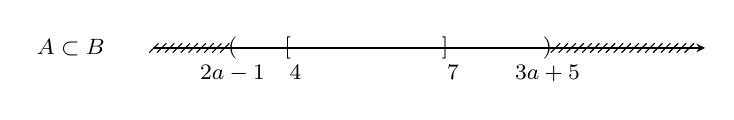
\begin{tikzpicture}[scale=1,>=stealth, font=\footnotesize, line join=round, line cap=round]
					\draw [-stealth] (0,0)--(7,0);
					\path (1,0) node{$($} (1,-0.1)node[below]{$2a-1$} (-.5,0)node[left]{$A \subset B$};
					\path (5,0) node{$)$} (5,-0.1)node[below]{$3a+5$};
					\path (1.7,0) node{$[$} (1.8,-0.1)node[below]{$4$};
					\path (3.7,0) node{$]$} (3.8,-0.1)node[below]{$7$};
					\foreach \x in{0,0.1,...,1} \draw (\x,0)--++(45:.08) (\x,0)--++(-135:.08);
					\foreach \x in{5.1,5.2,...,6.8} \draw (\x,0)--++(45:.08) (\x,0)--++(-135:.08);
				\end{tikzpicture}
			\end{center}
			\item Điều kiện tập $B$ khác tập rỗng: $2 a-1<3 a+5 \Leftrightarrow a>-6$\, \hfill{(1)}
			\item $A \subset B \Rightarrow \heva{& 2a-1<4 \\& 3a+5 \geqslant 7 } \Leftrightarrow \heva{& a<\dfrac{5}{2} \\& a \geqslant \dfrac{2}{3}} \Leftrightarrow \dfrac{2}{3} \leqslant a<\dfrac{5}{2}.$ \, \hfill{(2)}
			\item Kết hợp $(1)$ và $(2)$, ta được $\dfrac{2}{3} \leqslant a<\dfrac{5}{2}$.
			\item Xét các giá trị $a \in \mathbb{Z} \Rightarrow S=\{1 ; 2\}$.
			\item Có $4$ tập con của $S$ là $\varnothing $; $\{1\} $; $\{2\}$ và $S=\{1 ; 2\}$.
		\end{itemize}
	}
\end{bt}

%=== Câu 18 (ID: None) ===%

\nguon{nhóm Latex}
\dang{Ôn tập đề  1}
\begin{bt}
	Cho hai tập hợp khác rỗng $A=(1;5)$ và $B=(m;4m-1) \neq \varnothing$, $m \in \mathbb{R}$. Có bao nhiêu giá trị nguyên của tham số $m$ để $B \subset A$.
	\shortans{1}
	\loigiai{
		Vẽ trục số thể hiện $B \subset A$.
		\begin{center}
			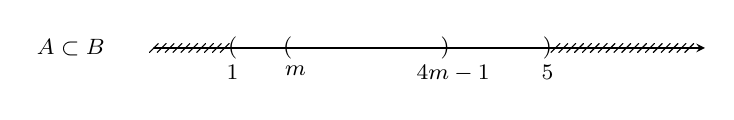
\begin{tikzpicture}[scale=1,>=stealth, font=\footnotesize, line join=round, line cap=round]
				\draw [-stealth] (0,0)--(7,0);
				\path (1,0) node{$($} (1,-0.1)node[below]{$1$} (-.5,0)node[left]{$A \subset B$};
				\path (5,0) node{$)$} (5,-0.1)node[below]{$5$};
				\path (1.7,0) node{$($} (1.8,-0.1)node[below]{$m$};
				\path (3.7,0) node{$)$} (3.8,-0.1)node[below]{$4m-1$};
				\foreach \x in{0,0.1,...,1} \draw (\x,0)--++(45:.08) (\x,0)--++(-135:.08);
				\foreach \x in{5.1,5.2,...,6.8} \draw (\x,0)--++(45:.08) (\x,0)--++(-135:.08);
			\end{tikzpicture}
		\end{center}
		Để $B \neq \varnothing $ thì $m<4 m-1 \Leftrightarrow m>\dfrac{1}{3}.~\hfill{(1)}$\\
		Và 
		$B\subset A 
		\Rightarrow \heva{&m \geq 1\\&4m-1\leq 5} 
		\Leftrightarrow 1 \leq m \leq \dfrac{3}{2}.~\hfill{(2)}$\\
		Từ $(1)$, $(2)$ suy ra $1 \leq m \leq \dfrac{3}{2}$.\\
		Vậy có $1$ giá trị nguyên của $m$ thì $B \subset A$.
	}
\end{bt}

%=== Câu 19 (ID: None) ===%

\nguon{nhóm Latex}
\dang{Ôn tập đề  1}
\begin{bt}
	Cho $2$ tập khác rỗng $A=(m-1 ; 4]$; $B=(-2 ; 2 m+2)$, $m \in \mathbb{R}$. Tìm $m$ nguyên dương để $A \subset B$.
	\loigiai{
		Vẽ trục số thể hiện $A \subset B$.
		\begin{center}
			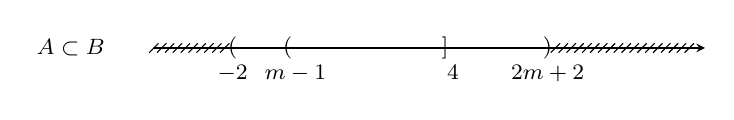
\begin{tikzpicture}[scale=1,>=stealth, font=\footnotesize, line join=round, line cap=round]
				\draw [-stealth] (0,0)--(7,0);
				\path (1,0) node{$($} (1,-0.1)node[below]{$-2$} (-.5,0)node[left]{$A \subset B$}; 
				\path (5,0) node{$)$} (5,-0.1)node[below]{$2m+2$};
				\path (1.7,0) node{$($} (1.8,-0.1)node[below]{$m-1$};
				\path (3.7,0) node{$]$} (3.8,-0.1)node[below]{$4$};
				\foreach \x in{0,0.1,...,1} \draw (\x,0)--++(45:.08) (\x,0)--++(-135:.08);
				\foreach \x in{5.1,5.2,...,6.8} \draw (\x,0)--++(45:.08) (\x,0)--++(-135:.08);
			\end{tikzpicture}
		\end{center}
		Với $2$ tập khác rỗng $A$, $B$ ta có điều kiện $ \heva{&m-1<4 \\&2m+2>-2} 
		\Leftrightarrow \heva{&m<5\\&m>-2}
		\Leftrightarrow-2<m<5$.\\
		Để $A \subset B 
		\Leftrightarrow \heva{& m-1 \geqslant-2 \\& 2 m+2>4} 
		\Leftrightarrow \heva{& m \geqslant-1 \\& 2 m+2>4} 
		\Leftrightarrow \heva{& m \geqslant-1 \\& m>1} 
		\Leftrightarrow m>1$.\\
		So với điều kiện $\Rightarrow 1<m<5$. Do đó có $3$ giá trị nguyên của $m$ thỏa mãn $A \subset B$.
	}
\end{bt}

%=== Câu 20 (ID: None) ===%

\nguon{nhóm Latex}
\dang{Ôn tập đề  1}
\begin{ex}
	Lớp $10 B_1$ có $7$ học sinh giỏi Toán, $5$ học sinh giỏi Lý, $6$ học sinh giỏi Hóa, $2$ học sinh chỉ giỏi Toán và Lý, $3$ học sinh chỉ giỏi Toán và Hóa, $1$ học sinh chỉ giỏi cả Lý và Hóa, $1$ học sinh giỏi cả $3$ môn Toán, Lý, Hóa.
	\choiceTF
	{\True Số học sinh chỉ giỏi môn Toán là $1$ học sinh}
	{\True Số học sinh chỉ giỏi môn Lý là $1$ học sinh}
	{Số học sinh chỉ giỏi môn Hóa là $2$ học sinh}
	{\True Số học sinh giỏi ít nhất một môn (Toán, Lý, Hóa) là $10$ học sinh}
	\loigiai{
		Gọi $T$, $L$, $H$ lần lượt là tập hợp các học sinh của lớp giỏi Toán, Lý, Hóa.\\
		Theo đề bài ta có: $|T|=7$; $|L|=5$; $|H|=6$; $|T \cap L|=3$; $|T \cap H|=4$; $|L \cap H|=2$; $|T \cap L \cap H|=3$.
		\begin{itemchoice}
			\item Số học sinh chỉ giỏi môn Toán $7-3-1-2=1$.
			\item Số học sinh chỉ giỏi môn Lý $5-1-1-2=1$.
			\item Số học sinh chỉ giỏi môn Hóa $6-3-1-1=1$.
			\item Số học sinh giỏi ít nhất một môn (Toán, Lý, Hóa) là: $1+2+1+1+1+3+1=10$.
	\end{itemchoice}}
\end{ex}

%=== Câu 21 (ID: None) ===%

\nguon{nhóm Latex}
\dang{Ôn tập đề  1}
\begin{bt}
	Cho tập hợp $A=(0 ;+\infty)$ và $B=\left\{x \in \mathbb{R} \mid m x^2-6 x+m-8=0\right\}$, $m$ là tham số. Xác định $m$, biết rằng tập $B$ có đúng hai tập con và $B \subset A$.
	\loigiai{
		Vì tập $B$ có đúng hai tập con nên $B$ có đúng $1$ phần tử. Do đó phương trình $m x^2-6x+m-8=0$ có duy nhất một nghiệm.
		\begin{enumerate}[TH1.]
			\item $m=0$ thì $x=-\dfrac{4}{3} 
			\Rightarrow B=\left\{-\dfrac{4}{3}\right\} \not\subset A$.
			\item $m \neq 0$ thì phương trình có nghiệm duy nhất\\
			$\Leftrightarrow \Delta'=0$
			$\Leftrightarrow 9-m(m-8)=0$
			$\Leftrightarrow-m^2+8 m+9=0$
			$\Leftrightarrow \hoac{& m=-1 \\& m=9.}$ 
			\begin{itemize}
				\item Với $m=-1 \Rightarrow B=\{-3\} \not\subset A$.
				\item Với $m=9 \Rightarrow B=\left\{\dfrac{1}{3}\right\} \subset A$.
			\end{itemize}
			Kết hợp với điều kiện $B \subset A$ ta có $m=9$.
		\end{enumerate}
	}
\end{bt}
